%%%%%%%%%%%%%%%%%%%%%%%%%%%%%%%%%%%%%%%%%
% Arsclassica Article
% LaTeX Template
% Version 1.1 (1/8/17)
%
% This template has been downloaded from:
% http://www.LaTeXTemplates.com
%
% Original author:
% Lorenzo Pantieri (http://www.lorenzopantieri.net) with extensive modifications by:
% Vel (vel@latextemplates.com)
%
% License:
% CC BY-NC-SA 3.0 (http://creativecommons.org/licenses/by-nc-sa/3.0/)
%
%%%%%%%%%%%%%%%%%%%%%%%%%%%%%%%%%%%%%%%%%

%----------------------------------------------------------------------------------------
%	PACKAGES AND OTHER DOCUMENT CONFIGURATIONS
%----------------------------------------------------------------------------------------

\documentclass[
10pt, % Main document font size
a4paper, % Paper type, use 'letterpaper' for US Letter paper
oneside, % One page layout (no page indentation)
%twoside, % Two page layout (page indentation for binding and different headers)
headinclude,footinclude, % Extra spacing for the header and footer
BCOR5mm, % Binding correction
]{scrartcl}

\usepackage{amsmath}
\usepackage{algorithm}
\usepackage{algpseudocode}
\usepackage{cite}

\renewcommand{\algorithmicforall}{\textbf{for each}}

%%%%%%%%%%%%%%%%%%%%%%%%%%%%%%%%%%%%%%%%%
% Arsclassica Article
% Structure Specification File
%
% This file has been downloaded from:
% http://www.LaTeXTemplates.com
%
% Original author:
% Lorenzo Pantieri (http://www.lorenzopantieri.net) with extensive modifications by:
% Vel (vel@latextemplates.com)
%
% License:
% CC BY-NC-SA 3.0 (http://creativecommons.org/licenses/by-nc-sa/3.0/)
%
%%%%%%%%%%%%%%%%%%%%%%%%%%%%%%%%%%%%%%%%%

%----------------------------------------------------------------------------------------
%	REQUIRED PACKAGES
%----------------------------------------------------------------------------------------

\usepackage[
nochapters, % Turn off chapters since this is an article        
beramono, % Use the Bera Mono font for monospaced text (\texttt)
eulermath,% Use the Euler font for mathematics
pdfspacing, % Makes use of pdftex’ letter spacing capabilities via the microtype package
dottedtoc % Dotted lines leading to the page numbers in the table of contents
]{classicthesis} % The layout is based on the Classic Thesis style

\usepackage{arsclassica} % Modifies the Classic Thesis package

\usepackage[T1]{fontenc} % Use 8-bit encoding that has 256 glyphs

\usepackage[utf8]{inputenc} % Required for including letters with accents

\usepackage{graphicx} % Required for including images
\graphicspath{{Figures/}} % Set the default folder for images

\usepackage{enumitem} % Required for manipulating the whitespace between and within lists

\usepackage{lipsum} % Used for inserting dummy 'Lorem ipsum' text into the template

\usepackage{subfig} % Required for creating figures with multiple parts (subfigures)

\usepackage{amsmath,amssymb,amsthm} % For including math equations, theorems, symbols, etc

\usepackage{varioref} % More descriptive referencing

%----------------------------------------------------------------------------------------
%	THEOREM STYLES
%---------------------------------------------------------------------------------------

\theoremstyle{definition} % Define theorem styles here based on the definition style (used for definitions and examples)
\newtheorem{definition}{Definition}

\theoremstyle{plain} % Define theorem styles here based on the plain style (used for theorems, lemmas, propositions)
\newtheorem{theorem}{Theorem}

\theoremstyle{remark} % Define theorem styles here based on the remark style (used for remarks and notes)

%----------------------------------------------------------------------------------------
%	HYPERLINKS
%---------------------------------------------------------------------------------------

\hypersetup{
%draft, % Uncomment to remove all links (useful for printing in black and white)
colorlinks=true, breaklinks=true, bookmarks=true,bookmarksnumbered,
urlcolor=webbrown, linkcolor=RoyalBlue, citecolor=webgreen, % Link colors
pdftitle={}, % PDF title
pdfauthor={\textcopyright}, % PDF Author
pdfsubject={}, % PDF Subject
pdfkeywords={}, % PDF Keywords
pdfcreator={pdfLaTeX}, % PDF Creator
pdfproducer={LaTeX with hyperref and ClassicThesis} % PDF producer
} % Include the structure.tex file which specified the document structure and layout

\hyphenation{Fortran hy-phen-ation} % Specify custom hyphenation points in words with dashes where you would like hyphenation to occur, or alternatively, don't put any dashes in a word to stop hyphenation altogether

%----------------------------------------------------------------------------------------
%	TITLE AND AUTHOR(S)
%----------------------------------------------------------------------------------------

\title{\normalfont\spacedallcaps{Initial Report on Dynamic Subgraph Isomorphism on GPU}} % The article title

%\subtitle{Subtitle} % Uncomment to display a subtitle

\author{\spacedlowsmallcaps{Shreyas Phanse (CS16M045)}}% The article author(s) - author affiliations need to be specified in the AUTHOR AFFILIATIONS block

\date{} % An optional date to appear under the author(s)

%----------------------------------------------------------------------------------------

\begin{document}

%----------------------------------------------------------------------------------------
%	HEADERS
%----------------------------------------------------------------------------------------

\renewcommand{\sectionmark}[1]{\markright{\spacedlowsmallcaps{#1}}} % The header for all pages (oneside) or for even pages (twoside)
%\renewcommand{\subsectionmark}[1]{\markright{\thesubsection~#1}} % Uncomment when using the twoside option - this modifies the header on odd pages
\lehead{\mbox{\llap{\small\thepage\kern1em\color{halfgray} \vline}\color{halfgray}\hspace{0.5em}\rightmark\hfil}} % The header style

\pagestyle{scrheadings} % Enable the headers specified in this block

%----------------------------------------------------------------------------------------
%	TABLE OF CONTENTS & LISTS OF FIGURES AND TABLES
%----------------------------------------------------------------------------------------

\maketitle % Print the title/author/date block

\setcounter{tocdepth}{2} % Set the depth of the table of contents to show sections and subsections only

\tableofcontents % Print the table of contents

\listoffigures % Print the list of figures


%----------------------------------------------------------------------------------------
%	ABSTRACT
%----------------------------------------------------------------------------------------

\section*{Abstract} % This section will not appear in the table of contents due to the star (\section*)

In real world problems which are modeled as graphs, subgraph isomorphism is an important problem. Since this problem is NP-hard, it is not an easy task to find solutions for large graphs in a small amount of time. however, Recent works have been able to solve the problem in reasonable amount of time on specific real world datasets. Because of numerous applications of the problem in many data mining and pattern matching fields, the problem is well studied and different methods have been proposed in past years. Some of the state-of-the-art techniques for the same have been studied and discussed in upcoming sections. In recent years, with the development of parallel programming and GPUs\cite{book}, massive speedup can be achieved on execution of various computing tasks. Our objective is to exploit this to obtain even faster query outputs for large graphs.

%----------------------------------------------------------------------------------------
%	AUTHOR AFFILIATIONS
%----------------------------------------------------------------------------------------

\let\thefootnote\relax\footnotetext{\textit{Computer Science Department, IIT Madras}}


%----------------------------------------------------------------------------------------

\newpage % Start the article content on the second page, remove this if you have a longer abstract that goes onto the second page

%----------------------------------------------------------------------------------------
%	INTRODUCTION
%----------------------------------------------------------------------------------------

\section{Introduction}

Subraph isomorphism is used in many real world problems such as chemical compounds, social networks, and biological structures. Many real applications in bioinformatics, chemistry, and software engineering require efficient and effective management of graph structured data.

One of most important graph queries in graph databases is the subgraph isomorphism query. That is, given a query q and a data graph g, find all embeddings of q in g. This problem is NP-hard. Various popular algorithms that have tried to solve the problem in reasonable amount of time are discussed in upcoming sections.

\subsection{Problem Definition}
A graph $q$ is defined as $(V, E,L)$ where $V$ is the set of vertices, $E(\subseteq V \times V)$ is the set of edges, and $L$ is a label function that maps a vertex to a set of labels. Without loss of generality, all subgraph isomorphism algorithms can be easily extended to handle graphs whose edges have labels.

A graph $q$ = $(V, E,L)$ is isomorphic to a subgraph of a data graph $g = (V', E', L')$ if there is an injection (or an embedding) $M : V \rightarrow V$ such that, $\forall u \in V $, $L(u) \subseteq L' (M(u))$, and $\forall (u_i, u_j) \in E$, $(M(u_i), M(u_j)) \in E'$.\\
Now, the subgraph isomorphism problem is defined as follows: “Given a query graph q and a data graph g, find all distinct embeddings of q in g.” This is explained by the following example.

\begin{figure}[h]
\centering 
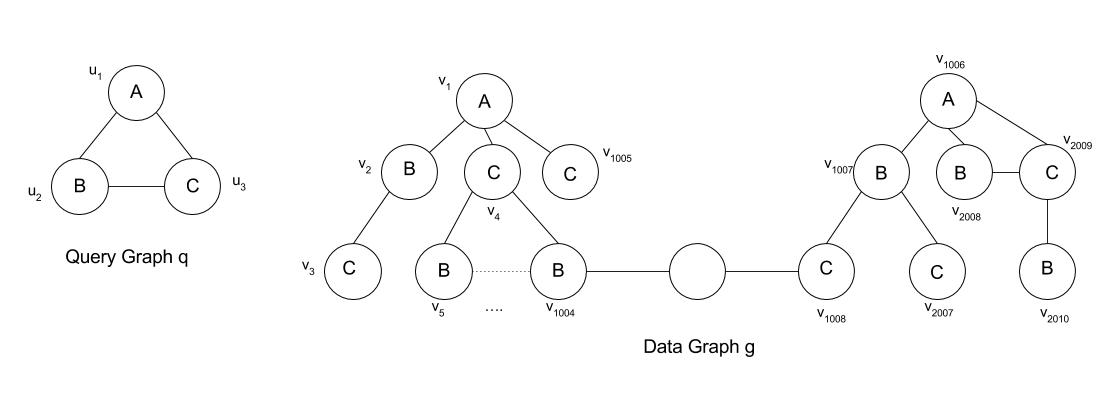
\includegraphics[width=\columnwidth]{problem_drawing} 
\caption[Subgraph Isomorphism]{A query graph $q$ and a data graph $g$} % The text in the square bracket is the caption for the list of figures while the text in the curly brackets is the figure caption
\label{fig:gallery} 
\end{figure}

For the above query graph, the data subgraph {$v_{1006}, v_{2008}, v_{2009}$} is isomorphic to the query graph and hence is a match. There is no other match for the given query graph in the data graph.\\

\textbf{Dynamic version:} In the dynamic version of subgraph isomorphism, the objective is to find distinct embeddings of query graph in the data graph where data graphs and query graphs modify structurally (i.e. edges get added/deleted from the graphs).\\
For example, for the above graph, we can remove an edge from the query graph as shown in the diagram below. The new matchings include all the previous matchings plus some other matchings. Our objective is to find the new matchings using the already found ones efficiently.

\subsection{Data Representation}
Graphs are represented as Compressed sparse rows\cite{csr}. The compressed sparse row (CSR) or compressed row storage (CRS) format represents a matrix M by three (one-dimensional) arrays, that respectively contain nonzero values, the extents of rows, and column indices. Hence given adjacency matrix of a graph, CSR representation can be obtained. This structure consumes very less space for large sparse graphs as compared to its adjacenct matrix. The following example shows an adjacency matrix (M) for graph in figure 2(a) and its CSR representation.\\

\[
    M =
    \begin{bmatrix}
        0 & 1 & 1 & 1 & 0 & 0 & 0 & 0 & 0\\
        1 & 0 & 0 & 0 & 1 & 1 & 1 & 0 & 0\\
        1 & 0 & 0 & 0 & 0 & 0 & 0 & 0 & 0\\
        1 & 0 & 0 & 0 & 0 & 0 & 0 & 0 & 0\\
        0 & 1 & 0 & 0 & 0 & 1 & 0 & 0 & 0\\
        0 & 1 & 0 & 0 & 1 & 0 & 0 & 1 & 0\\
        0 & 1 & 0 & 0 & 0 & 0 & 0 & 0 & 1\\
        0 & 0 & 0 & 0 & 0 & 1 & 0 & 0 & 0\\
        0 & 0 & 0 & 0 & 0 & 1 & 1 & 0 & 0\\
    \end{bmatrix}
\]
\[
    IA = 
    \begin{bmatrix}
        0 & 3 & 7 & 8 & 9 & 11 & 14 & 16 & 17 & 18
    \end{bmatrix}
\] 
\[
    JA =
    \begin{bmatrix}
        1 & 2 & 3 & 0 & 4 & 5 & 6 & 0 & 0 & \dots
    \end{bmatrix}
\]
Here, IA is an array of size rows(M) + 1 which is recursively defined as:
\begin{itemize}
    \item $IA[0] = 0$
    \item $IA[i]$ = $IA[i - 1]$ + number of non zero entries in $i - 1^{th}$ row of M
\end{itemize}
JA contains the column index of all the non zero entries in M in row major order.
%----------------------------------------------------------------------------------------
%	ALGOS
%----------------------------------------------------------------------------------------
\section{Algorithms}

Following section will give a brief overview on the few of the state-of-art algorithms\cite{comparision} for subgraph isomorphism.

\subsection{Generic Algorithm}

The generic subgraph isomorphism algorithm is implemented
as a backtracking algorithm which finds solutions
by incrementing partial solutions or abandoning them when
it determines they cannot be completed. Most of the popular algorithms are variations of the generic algorithm. It must be noted that the efficiency of algorithms depends on the heuristics used for pruning the candidate list and selecting the order of vertices that are to be matched.

\begin{algorithm}
\caption{\textsc{GenericAlgo}}\label{euclid}
\begin{algorithmic}[1]
%\textbf{Input:} Data graph g, Query graph q.\\
%\textbf{Output:} all subgraph isomorphisms of q in g.
\State $M \gets \emptyset$
\ForAll{$u \in V(q)$}
\State $C(u) \gets \textsc{FilterCandidates}(q, g, u...)$
\If{$c = \emptyset$}
\State \textbf{return}
\EndIf
\EndFor
\State $\textsc{SubgraphSearch}(q, g, M,...)$ 
\Procedure{$\textsc{SubgraphSearch}(q, g, M,...)$}{}
\If{$|M| = |V(q)|$}
    \State \textbf{report} M
    \Else
    \State $u \gets \textsc{NextQueryVertex}(..)$
    \State $C_R \gets \textsc{RefineCandidates}(...)$
    \ForAll{$V \in C_R$ such that v is not yet matched}
        \If{\textsc{IsJoinable}(q, g, M, u, v)}
            \State \textsc{UpdateState(M, u, v...)}
        \EndIf
    \EndFor
\EndIf
\EndProcedure
\end{algorithmic}
\end{algorithm}

Algorithm 1 shows a generic subgraph isomorphism algorithm, \textsc{GenericAlgo}. Its inputs are a query graph q and a data graph g, and its output is a set of subgraph isomorphisms (or embeddings) of q in g. Here, to represent an embedding, we use a list M of pairs of a query vertex and a corresponding data vertex. The specific implementations of these procedures have been discussed in the respective subsections.

%------------------------------------------------

\subsection{Ullmann Algorithm\cite{ullmann}}

Ullmann Algorithm exploits the template mentioned in Genric algorithm in the following way.\\
\\
\textsc{FilterCandidates:} \textsc{FilterCandidates} returns a set of data graph vertices with a matching label $u$. For example, in figure $1$, it will return candidates of $u_1$ as \{$v_1, v_{1006}$\}\\
\\
\textsc{NextQueryVertex:} returns one vertex at a time from the vertices in the order they appear in the input. It is clear that the performance of the Ullmann algorithm highly depends on the input order of the query vertices. This issue is discussed in the next subsection.\\
\\
\textsc{RefineCandidates:} prunes out all candidate vertices that have a smaller degree than u. In our running example, $v_{1005}$ will be pruned out as a candidate for $u_3$ because it has degree less than that of $u_3$ and hence can never map to it.\\
\\
\textsc{IsJoinable:} iterates through all adjacent query vertices of u. If there is an adjacent vertex already matched then it checks whether there is a corresponding edge in the data graph. In our running example, \{$u_1, u_2, u_3$\} will be matched to \{$v_1, v_2, v_3$\}. The \textsc{IsJoinable} procedure will check if there are corresponding edges between these matches. Since the edge between $v_2$ and $v_4$ is absent, the \textsc{IsJoinable} procedure will return false.

\subsection{VF2 algorithm\cite{vf2}}

\textsc{NextQueryVertex:} Unlike Ullmann, VF2 starts with the first vertex and selects a vertex connected from the already matched query vertices. Note that the original VF2 algorithm does not define any order in which query vertices are selected.\\
\\
\textsc{RefineCandidates:} VF2 uses the following three pruning
rules to prune out data vertex candidates:
\begin{enumerate}
    \item Prune out any vertex v in C(u) such that v is not connected from already matched data vertices.
    \item The number of unmatched vertices of neighbors of v in query graph must be greater than unmatched vertices of neighbors of u in data graph.
    \item The count of neighbors of v which are not the neighbors of mapped nodes and are not mapped nodes in Q must be greater than neighbors of u who are not neighbors of mapped nodes and are not mapped nodes in D.
\end{enumerate}

\subsection{$\boldsymbol{Turbo_{ISO}}$ Algorithm\cite{turbo}}

\begin{algorithm}
\caption{\textsc{$Turbo_{ISO}(g,q)$}}\label{euclid}
\begin{algorithmic}[1]
%\textbf{Input:} Data graph g, Query graph q.\\
%\textbf{Output:} all subgraph isomorphisms of q in g.
\State $u_s \gets \textsc{ChooseStartQueryVertex(q,g)}$
\State $q' \gets \textsc{ReWriteToNECTree}(q,u_s)$ // q': NEC Tree
\ForAll{$v_s$ in {$v|(v \in V(g))$ and $(L(u_s) \subseteq L(v))$}}
    \If{$\textsc{ExploreCR}(u'_s,{v_s},CR)=FAIL$}
        \State \textbf{continue}
    \EndIf
    \State order = $\textsc{DetermineMatchingOrder}(q',CR)$
    \State $\textsc{UpdateState}(M,F,{us},{vs})$
    \State $\textsc{SubGraphSearch}(g,q',q,order)$
    \State $\textsc{RestoreState}(M,F,{u_s},{v_s})$
\EndFor
\end{algorithmic}
\end{algorithm}

\begin{figure}[H]
\centering 
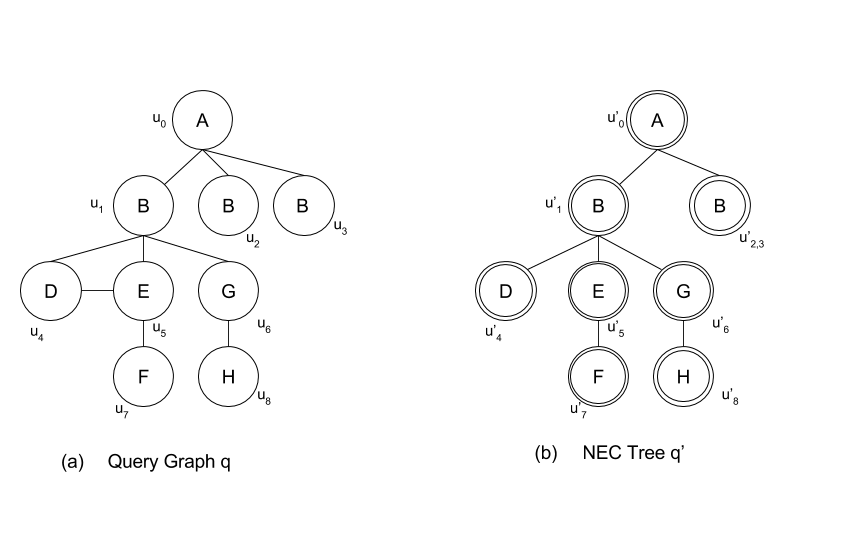
\includegraphics[scale=0.5]{Figures/123.png} 
\caption[Query graph and NEC Tree]{A query graph and its corresponding NEC Tree} % The text in the square bracket is the caption for the list of figures while the text in the curly brackets is the figure caption
\label{fig:gallery} 
\end{figure}


$Turbo_{ISO}$ uses the concept of Neighbourhood Equivalence Class (NEC). Each query vertex in the same NEC has identically matching data vertices. Matching time can be reduced using this concept as number of vertices that are to be matched will be reduced. Figure 2 shows a query graph and it's equivalent NEC tree.

\newpage
%------------------------------------------------



%----------------------------------------------------------------------------------------
%	SUGGESTED SOLUTION AND IMPLEMENTATION
%----------------------------------------------------------------------------------------

\section{Suggested solution and Implementation}

The Dynamic version of the problem can be split into the following subproblems:

\begin{enumerate}
    \item No change in either graphs: This is the static version.
    \item Edge added to query graph: In this case, new matchings will be a subset of the previous matchings. So the search space can be reduced to the previous matchings itsef.
    \item Edge deleted from query graph: Proposed solution for this case is to maintain matching for a few selected subgraphs of the query graph. If the modified query graph is a supergaph of any of the stored matchings, the search space is reduced.
    \item Edge removed from the data graph: This same as case 2. New matchings will be a subset of the previous matchings. So same approach can be used.
    \item Edge added to the data graph: This case is yet to be explored.
\end{enumerate}

\renewcommand{\refname}{\spacedlowsmallcaps{References}} % For modifying the bibliography heading
\bibliographystyle{unsrt}
\bibliography{Figures/reated.bib}

\end{document}
